\documentclass[tikz,border=3pt]{standalone}
\usepackage{libertine}
\usetikzlibrary{arrows.meta,positioning}
\definecolor{navy}{HTML}{183A61}
\definecolor{blue}{HTML}{377EB8}
\definecolor{bluefill}{HTML}{EAF3FB}
\definecolor{orange}{HTML}{D07820}
\definecolor{orangefill}{HTML}{FFF3E5}
\definecolor{green}{HTML}{4F8A68}
\definecolor{greenfill}{HTML}{EEF8F1}
\definecolor{slate}{HTML}{66778B}
\definecolor{grayfill}{HTML}{F5F7FA}
\tikzset{
  panel/.style={rounded corners=4pt, draw=slate, fill=white, line width=.8pt},
  opbox/.style={rounded corners=2pt, draw=blue, fill=bluefill, line width=.75pt,
    text width=3.75cm, minimum height=7.5mm, align=center, font=\scriptsize\bfseries, text=navy},
  control/.style={opbox, draw=orange, fill=orangefill, text=orange},
  state/.style={opbox, draw=slate, fill=grayfill},
  visible/.style={opbox, draw=green, fill=greenfill, text=green},
  arr/.style={-{Stealth[length=2mm]}, draw=slate, line width=.85pt},
  hb/.style={font=\tiny\itshape, text=orange, fill=white, inner sep=1pt}
}
\begin{document}
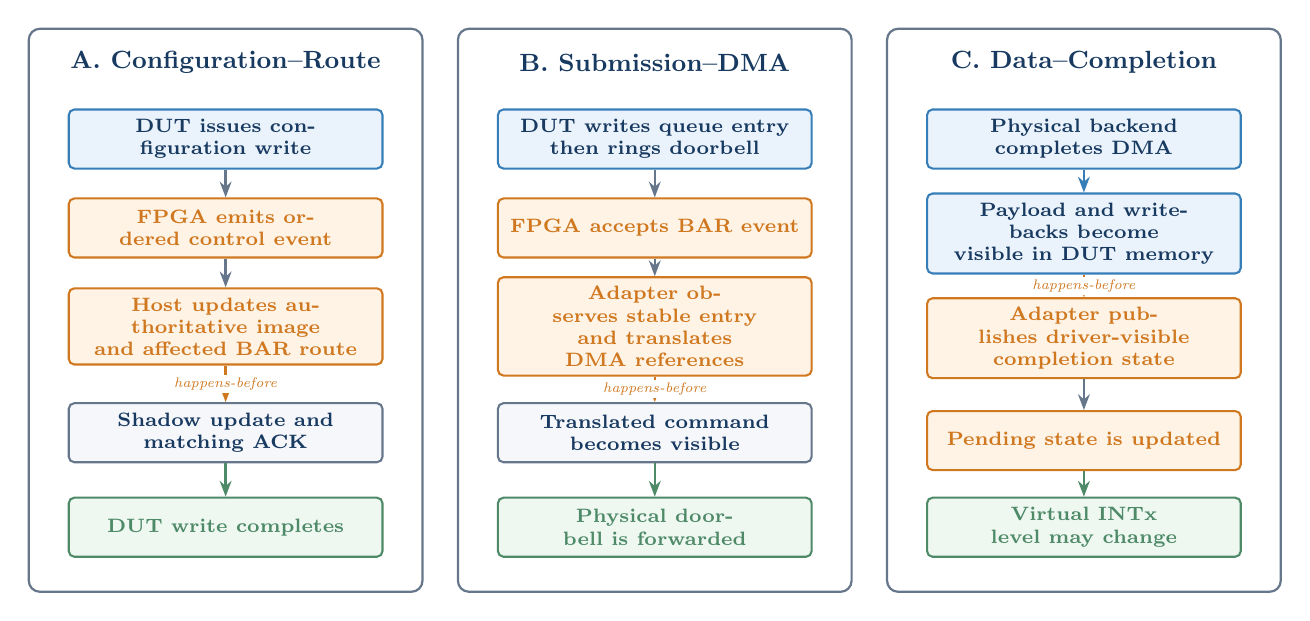
\begin{tikzpicture}[x=1cm,y=1cm]
  \foreach \x in {0,5.45,10.9} {
    \fill[white, rounded corners=4pt] (\x,0) rectangle ++(5.0,7.15);
    \draw[slate, line width=.8pt, rounded corners=4pt] (\x,0) rectangle ++(5.0,7.15);
  }
  \node[font=\small\bfseries, text=navy] at (2.5,6.72) {A. Configuration--Route};
  \node[font=\small\bfseries, text=navy] at (7.95,6.72) {B. Submission--DMA};
  \node[font=\small\bfseries, text=navy] at (13.4,6.72) {C. Data--Completion};

  \node[opbox] (a1) at (2.5,5.75) {DUT issues configuration write};
  \node[control] (a2) at (2.5,4.62) {FPGA emits ordered control event};
  \node[control] (a3) at (2.5,3.37) {Host updates authoritative image\\and affected BAR route};
  \node[state] (a4) at (2.5,2.02) {Shadow update and matching ACK};
  \node[visible] (a5) at (2.5,.82) {DUT write completes};
  \draw[arr] (a1)--(a2); \draw[arr] (a2)--(a3);
  \draw[arr, draw=orange] (a3)--node[hb]{happens-before}(a4);
  \draw[arr, draw=green] (a4)--(a5);

  \node[opbox] (b1) at (7.95,5.75) {DUT writes queue entry\\then rings doorbell};
  \node[control] (b2) at (7.95,4.62) {FPGA accepts BAR event};
  \node[control] (b3) at (7.95,3.37) {Adapter observes stable entry\\and translates DMA references};
  \node[state] (b4) at (7.95,2.02) {Translated command becomes visible};
  \node[visible] (b5) at (7.95,.82) {Physical doorbell is forwarded};
  \draw[arr] (b1)--(b2); \draw[arr] (b2)--(b3);
  \draw[arr, draw=orange] (b3)--node[hb]{happens-before}(b4);
  \draw[arr, draw=green] (b4)--(b5);

  \node[opbox] (c1) at (13.4,5.75) {Physical backend completes DMA};
  \node[opbox] (c2) at (13.4,4.55) {Payload and writebacks become\\visible in DUT memory};
  \node[control] (c3) at (13.4,3.22) {Adapter publishes driver-visible\\completion state};
  \node[control] (c4) at (13.4,1.92) {Pending state is updated};
  \node[visible] (c5) at (13.4,.82) {Virtual INTx level may change};
  \draw[arr, draw=blue] (c1)--(c2);
  \draw[arr, draw=orange] (c2)--node[hb]{happens-before}(c3);
  \draw[arr] (c3)--(c4); \draw[arr, draw=green] (c4)--(c5);
\end{tikzpicture}
\end{document}
